\documentclass[10pt,aspectratio=169]{beamer}

\usepackage{amsmath}

\usepackage{mypresento/config/presento}
\usepackage{tikz}
\usetikzlibrary{shadings,shadows,calc,backgrounds,positioning}
\usepackage{tcolorbox}
\usepackage{adjustbox}
\usepackage{bytefield}
\newcommand{\colorbitbox}[3]{%
    \rlap{\bitbox{#2}{\color{#1}\rule{\width}{\height}}}%
    \bitbox{#2}{#3}}
\tcbuselibrary{skins,breakable}

\usepackage{caption}

\usepackage[caption=false]{subfig}
%\usepackage{transparent}
%\setbeameroption{show notes}

\usepackage[backend=bibtex,style=phys]{biblatex}
\bibliography{bib/myrefs}

\definecolor{darkblue}{HTML}{000099}
\usepackage{listings}
\lstset{
    frameround=fttt,
    language=C,
    numbers=left,
    %stepnumber=5,               % Abstand zwischen den Zeilennummern       
    %numberfirstline=false
    breaklines=true,
    keywordstyle=\color{black}\bfseries, 
    basicstyle=\ttfamily\footnotesize\color{darkblue},
    showstringspaces=false,
    numberstyle=\color{black},
	tabsize=2,
	columns=flexible,
	keepspaces=true
    }
\lstMakeShortInline[columns=fixed]|

% figures
\usepackage {pgf}                                 % includepgf for bitmaps
\usepackage{graphicx}

% Information
\title{Extending Compiler Support for the BrainScaleS Plasticity Processor}
\subtitle{Bachelor's Thesis Presentation}
\author{Arthur Heimbrecht}
\institute{}
\date{\today}

\begin{document}


% Title page
{
\usebackgroundtemplate{
    \tikz[overlay, remember picture]\node[opacity=0.3, inner sep=0, outer sep=0, ] at (current page.center) {\includegraphics[width=\paperwidth]{pictures/dls_die_photo.jpg}};
}
\begin{frame}[plain]
\maketitle
\note{ Welcome everybody to this talk about my Bachelor thesis. For some this might be a quite technical talk,so feel free to ask questions even during the presentation.
The title of my thesis was Extending Compiler Support for the BrainScaleS Plasticity Processor.}
\end{frame}

}

\begin{frame}{Contents}
\begin{columns}[c]
    \begin{column}{.5\textwidth}
        \begin{minipage}[t][0.5\textheight]{0.75\textwidth}
            \tableofcontents[sectionstyle=show, subsectionstyle=show/show/shaded]
        \end{minipage}\hfill
    \end{column}

    \begin{column}{.5\textwidth}
        \centering
        \begin{figure}
            \includegraphics[width=\textwidth]{pictures/dls_die_photo.jpg}
            \caption{\label{fig:dls} Photograph of HICANN-DLS chip, \citeauthor{PPU}}
        \end{figure}
    \end{column}
\end{columns}
\note{
    As the title hints there are two main components to this talk, which are the plasticity processing unit, or short PPU, and Compilers, specifically GCC.
    I will briefly talk about both of these and their applications.
    Afterwards I will explain, what I did during my thesis, which is of course followed by a short presentation of the results with an outlook as well.

    But first I should explain, what the PPU is.
}
\end{frame}

% sections in the presentation
\section{PPU Architecture}
\begin{frame}{HICANN-DLS}
    \begin{columns}[c]
    \begin{column}{0.5\textwidth}
        \centering
        \begin{figure}
                \begin{adjustbox}{center, max width={.40\columnwidth}}
                    
\noindent{\begin{minipage}{\textwidth}
   
\begin{tikzpicture}[style={circle,draw,fill=black,minimum size=15}, line width=.5mm]
       \foreach \x in {0,...,31}
           \foreach \y in {0,...,31} 
                  {\pgfmathtruncatemacro{\label}{\x - 5 *  \y +21}
                  \node [circle,draw,fill=black,minimum size=0.1, inner sep = 0pt]  (\x\y) at (0.3*\x,0.3*\y) {};}
   \end{tikzpicture}
\end{minipage}}

                \end{adjustbox}
            \caption{\label{fig:array} Schematic Representation of the Synapse Array on HICANN-DLS}
        \end{figure}

    \end{column}

    \begin{column}{0.5\textwidth}
        \centering
        \begin{figure}
            \includegraphics[width=\textwidth]{pictures/dls_marked.pdf}
            \caption{\label{fig:dls} Photograph of the HICANN-DLS Chip, modified from \citeauthor{PPU}}
        \end{figure}
    \end{column}
    \note{\tiny
        I am assuming that everybody here likely has heard about the HICANN-DLS.
        In short it is a chip that emulates neural networks through neurons and synapses that are implemented directly on the chip.
        What is special about the DLS, is the addition of a PPU to the HICANN system.
        The PPU is capable of performing simple computation and allows for on-line plasticity directly on the chip itself.

        As you can see to the right I have taken the previous picture of the HICANN-DLS chip and marked the physical compartments.
        The PPU actually takes up a large space on the chip but before I am going to talk about the PPU, I will talk about the other parts briefly
        First we have the neurons.
        There are 32 neurons on the HICANN-DLS and each neuron is a circuit that receives some input signal which can cause the neurons to spike.
        These signals come from the so called synapse array-which is to the left.
        It connects 32 pre-synaptic inputs to all 32 neurons down here.
        This gives a total of 1024 synapses on each HICANN-DLS.
        
        Each synapse is realized through a circuit that takes the input signal and modifies it with a synpatic weight, that is saved in each synapse.
		You can see a representation of this weight on whiteboard.
        There are also other properties to each synapse, which are partly handled by first two bits, but for this presentation it is enough to focus on the synaptic weights.
        Each synaptic weight is 6 bits wide, as you can see, which is equivalent to numbers between 0 and 63 or a fixed-point number with an accuracy of $2^{-6}$.
		<bild whiteboard>
        
        The pre-synaptic inputs are handled by an FPGA, that takes care of spike routing.
        
        But there is also a correlation analog digital converter, that receives signals from synapses if a signal is forwarded to neurons.
        Through the CADC one can read out correlation that can be used for plasticity by the PPU.

        The PPU is this remaining large section of the HICANN-DLS chip.
		Most of this is based on an existing processor architecture, that is called POWER architecture, but it was extended with a custom vector extension which we will call s2pp.

		In general it is good to keep this in mind during my talk and I also noted it on the whiteboard:
		The processing unit in HICANN DLS is called the PPU, the architecture with the vector extension is called nux architecture and the vector extension will be called s2pp.
		There is no fixed convention and some might use it differently, I just wanted to clarify this.

		Now I want to talk a little about processors in general and apply this to the PPU.
}
    \end{columns}
\end{frame}

\begin{frame}{Plasticity Processing Unit}
    \begin{columns}[c]
    \begin{column}{0.5\textwidth}
		\begin{itemize}[<1->]
			\setlength\itemsep{1em}
            \item ``Common'' von-Neumann architecture
			\item Machine Instructions
            \item Arithmetic Logic Unit (ALU)
            \item<2-> $\textrm{latency}(\textrm{register}) \ll \textrm{latency}(\textrm{memory}) $
		\end{itemize}
    \end{column}

    \begin{column}{0.5\textwidth}
        \centering
        \vspace*{3em}
        \begin{figure}
                \begin{adjustbox}{center, max width={.7\columnwidth}}
                    \chapter{Processor basics}
\label{chapter:processor}

Next to all processors used these days are built upon the so called von-Neumann architecture \todo{add reference}.
\todo{cite freidmann dissertation}Though the main goal of this group is to provide an alternative analogue architecture that is inspired by nature, there are advantages to the classic model of processors which are needed at some point.
The main advantage of digital systems over analogue systems such as the human brain, is the ability to do calculations at much higher speeds.
For this reason ``normal" processors are responsible for handling experiment data as well as setting up different parts of the experiment.
One such task is applying learning rules to the synapses during or in between experiments which can either be done by hand or with the help of the aforementioned PPU.
The second option is especially valuable when updating synaptic weights during an experiment as the PPU does this much faster than a system which interacts from the outside.
This is important for achieving experimental speeds that are $10^{4}$ times faster than their biological counterparts.

Therefore the PPU is one of many von-Neumann processors in this world and follows the same basic concepts.
It is important to understand these concepts as they build the foundation to this report!



ALU
FPU
memory
memory controller
clockcycle
pipeline


                \end{adjustbox}
            \caption{\label{fig:processor} Schematic of General Purpose Processor with von-Neumann Architecture}
        \end{figure}
    \end{column}
    \end{columns}
\note{	
		As you may know, next to all computing nowadays is done by processors which are often described as CPUs.
		The processors are normally built according to the von-Neumann architecture, which combines programs and data in the same memory.
		The processor fetches so called machine instructions from the memory and analyzes them to decide what to do.
		This is running a program.
		Most instructions get passed to the Arithmetic Logic Unit, or just ALU, that performs any sort of computation in the processor.
		To do this, the ALU has access to so called registers.
		These registers can hold small amounts of data, usually one variable, but offer a very low access time.
		The ALU uses these registers for computation and saves results there as well.
		Data is then written separately into memory and new values for registers are loaded from memory.
		Using memory usually takes a significant amount of time longer than access to registers and thus, programs try to use registers as much as possible.
}

\end{frame}

\begin{frame}{PPU Architecture}
    \begin{columns}[c]
    \begin{column}{0.5\textwidth}
        \begin{itemize}
			\setlength\itemsep{1em}
			\item Based on POWER architecture
            \item Vector Extension \\ \hspace{10mm}
				$\rightarrow$ Parallelization \\ \hspace{10mm}
				$\rightarrow$ Performance
            \item Weight Updates
			\item Access to Synaptic Array
        \end{itemize}
    \end{column}

    \begin{column}{0.5\textwidth}
        \centering
        \begin{figure}
            \includegraphics[width=.8\textwidth]{pictures/nux.pdf}
            \caption{\label{fig:nux} Structure of nux Architecture}
        \end{figure}
    \end{column}
    \end{columns}
\note{	
		Instead of the ALU, some instructions can be passed to other units that can perform special instructions.
		These units may also use different kinds of registers.

		And this is the case for the PPU.
		It includes a custom vector extension with special vector registers.
		Using vector registers is favorable for operations that use have to be applied to multiple values, but can be done in parallel.
		This works because and operation is performed on all vector elements the same way.
		
		And this is the strength of the PPU as is allows to compute weight updates for up to 16 synapses at the same time, which increases performance significantly. 
		For this reason the PPU is also connected to the synaptic array and is able to read out and write synaptic weights, in form of those 8 bits on the whiteboard.
		Esspecially it can do this vector-wise as well.

		Although it induces a problem because the vector unit uses special instructions that are unique to the nux architecture.
}
\end{frame}



\section{GCC Structure}
\begin{frame}[fragile]{Compiler Structure}
    \begin{columns}[c]
    \begin{column}{0.5\textwidth}
        \begin{itemize}
			\setlength\itemsep{1em}
            \item Program $\xrightarrow{\text{compile}}$ Executable
			\item Compiling Stages
			\item Compiler $\rightarrow$ Assembly
			\item Back-End is target-dependent
        \end{itemize}
    \end{column}

    \begin{column}{0.5\textwidth}
        \centering
        \begin{figure}
            \begin{adjustbox}{center, max width={.6\columnwidth}}
				    \tcbset
    {my box/.style={enhanced,colframe=blue!70!black,colback=white!50!blue,colupper=red!50!black,
        fonttitle=\bfseries,nobeforeafter,center title, noparskip, size=small},
    every box on layer 1/.style={every box},
    every box on layer 2/.style={reset,my box}}
\begin{tcolorbox}[enhanced jigsaw, width=\textwidth, opacityframe=0.0, opacityback=0.0]
\begin{tcolorbox}[enhanced, height=.5cm, width=\linewidth, remember as=pp, opacityframe=0.0, opacityback=0.0]\end{tcolorbox}
\begin{tcolorbox}[enhanced, height=.7cm, width=\linewidth, watermark text=Preprocessor, remember as=pp]\end{tcolorbox}
\begin{tcolorbox}[tcbox raise base, width=\linewidth, enhanced jigsaw, remember as=cmp]
    \begin{tcolorbox}[enhanced, breakable, noparskip,opacityframe=0.3, opacityback=0.3, height=1.4cm, width=\linewidth, watermark text=Front-End, remember as=fe]
    \end{tcolorbox}
    \begin{tcolorbox}[enhanced, breakable, noparskip,opacityframe=0.3, opacityback=0.3, height=0.7cm, width=\linewidth, watermark text=Middle-End, remember as=me]
    \end{tcolorbox}
    \begin{tcolorbox}[enhanced, breakable, noparskip,opacityframe=0.3, opacityback=0.3, height=1.1cm, width=\linewidth, watermark text=Back-End, remember as=be]
    \end{tcolorbox}
\end{tcolorbox}

\end{tcolorbox}

\begin{tikzpicture}[overlay,remember picture,line width=1mm]
    \draw[->, shorten >=-1.5mm] ($(pp.north)+(0,1.5)$) -- node [left] {program code} (pp.north);
    \draw[->, shorten >=-1.5mm] (pp.south) -- (fe.north);
    \draw[->, shorten >=-1.5mm] (fe.south) -- (me.north);
    \draw[->, shorten >=-1.5mm] (me.south) -- (be.north);
    \draw[->] (be.south) -- node [left] {machine files} ++(0,-1.5);
\end{tikzpicture}

				
    \tcbset
    {enhanced,colframe=blue!70!black,colback=white!50!blue,colupper=red!50!black,
    fonttitle=\bfseries,nobeforeafter,center title, noparskip}
            \begin{tcolorbox}[tcbox raise base, width=\linewidth, enhanced jigsaw, remember as=cp]
                \begin{tcolorbox}[enhanced jigsaw, breakable, noparskip,opacityframe=0.3, opacityback=0.3, width=\linewidth]
                    \begin{tcolorbox}[enhanced,center title,width=\linewidth, remember as=sc]
                        \begin{center}Scanner\end{center}
                    \end{tcolorbox}
                    \begin{tcolorbox}[enhanced,width=\linewidth, remember as=ps]
                        \begin{center}Parser\end{center}  
                    \end{tcolorbox}
                    \begin{tcolorbox}[enhanced, width=\linewidth, remember as=sa]
                        \begin{center}Semantic \\ Analyzer \end{center} 
                    \end{tcolorbox}
                    \begin{tcolorbox}[enhanced, width=\linewidth, remember as=sco]
                        \begin{center}Source Code \\ optimizer \end{center}
                    \end{tcolorbox}
                \end{tcolorbox}
                \begin{tcolorbox}[enhanced jigsaw, breakable, noparskip,opacityframe=0.3, opacityback=0.3, height=1cm, width=\linewidth, remember as=me, watermark text=Middle-End]
                \end{tcolorbox}
                \begin{tcolorbox}[enhanced jigsaw, breakable, noparskip,opacityframe=0.3, opacityback=0.3, width=\linewidth]
                    \begin{tcolorbox}[enhanced, width=\linewidth, remember as=cg]
                        \begin{center}Code Generator  \end{center}
                    \end{tcolorbox}
                    \begin{tcolorbox}[enhanced, width=\linewidth, remember as=tco]
                        \begin{center}Target Code \\ Optimizer \end{center}
                    \end{tcolorbox}
                \end{tcolorbox}
            \end{tcolorbox}
            \begin{tikzpicture}[overlay,remember picture,line width=1mm]
                \draw[->, shorten >=-1.5mm] ($(cp.north)+(0,1)$) -- (sc.north);
                \draw[->, shorten >=-1.5mm] (sc.south) -- (ps.north);
                \draw[->, shorten >=-1.5mm] (ps.south) -- (sa.north);
                \draw[->, shorten >=-1.5mm] (sa.south) -- (sco.north);
                \draw[-] (sco.south) -- (me.north);
                \draw[->, shorten >=-1.5mm] (me.south) -- (cg.north);
                \draw[->, shorten >=-1.5mm] (cg.south) -- (tco.north);
                \draw[->] (tco.south) -- ($(cp.south)+(0,-1)$);
            \end{tikzpicture}
            \begin{tikzpicture}[overlay,remember picture,line width=1mm]
                \draw[-, draw=blue!30!white,line width=.5mm, shorten >=.2cm,shorten <=.1cm] (cmp.north east) -- (cp.north west);
                \draw[-, draw=blue!30!white,line width=.5mm, shorten >=.2cm,shorten <=.1cm] (cmp.south east) -- (cp.south west);
            \end{tikzpicture}

            \end{adjustbox}
            \caption{\label{fig:compiler} Structure of Compiling Process and Compiler}
        \end{figure}
    \end{column}
    \end{columns}
\note{	\scriptsize
		This is of special significance when using a compiler.
		But why?
		I am quite sure that all of you have use compilers regularly and generally know what they do.
		And most will probably say that a compiler compiles code, or to be more specific it converts a program into a file that the computer can run.
		This is of course right and is follows the definition of a compiler.
		But there is much more to this.
		
		What we usually call compiler consists of several compiling stages that follow different purposes, like the preprocessor.
		It takes care of substituting macros and including header files in program code.
		The actual compiler will then take the preprocessed code and create an assembly file from this.

		Assembly is a language that represents machine instructions which have specific names and render pretty much the lowest level of coding a human would do.
		Listing ... is an example of this and some might actually have seen this before.

		The assembly file, which is generated by the compiler then gets converted into pure machine code, hence no names only numbers, by the assembler and then is combined with other files and gets assigned a memory location by the linker and loader.
		
		But since I focused on the compiler in this thesis, I should also give an overview of the internal structure of a compiler as well.
		As you can see, there are different phases in the compiler and these also follow different purposes.
		But we only need to focus on the last two stages which are part of the back-end.
		
		The back-end is mainly responsible for creating the actual machine code, or assembly, from input by the front-end and the middle-end.
		It then also optimizes the code it generated, but specifically for one processor architecture.
		In general a back-end is always machine-dependent, with machine meaning a processor architecture, as the assembly language is different for various processor architectures.
		One architecture, that most of you might know is the ARM architecture that is at the heart of every smartphone and also SpiNNaker.

	The PPU though, is based on the POWER architecture, as I already mentioned.}
\end{frame}

\begin{frame}[fragile]{GCC for the PPU}
    \begin{columns}[c]
    \begin{column}{0.5\textwidth}
        \begin{itemize}
			\setlength\itemsep{1em}
            \item No ``official'' support for s2pp
			\item Currently using macros
			\item<3-> Existing AltiVec extension
			\item<4-> Intrinsics $\rightarrow$ \textbf{use this}
        \end{itemize}
    \end{column}

    \begin{column}{0.5\textwidth}
        \centering
		\begin{onlyenv}<1>
				\begin{lstlisting}[title=Example from ppu\_sweep.c]
...
/** Definitions for vector registers **/
#define VR_TMP     0
#define VR_CAUSAL  1
#define VR_ACAUSAL 2
#define VR_RST     3
#define VR_NULL_C  4

...
				\end{lstlisting}
	\end{onlyenv}

		\begin{onlyenv}<2->
				\begin{lstlisting}[title=Example of Macro Usage]
				...
  fxv_splatb(VR_TMP, 1);
  fxv_addbm(VR_TMP_1, VR_A, VR_TMP);
				\end{lstlisting}
	\end{onlyenv}

		\begin{onlyenv}<3->
				\begin{lstlisting}[title=Example of AltiVec]
				...
  tmp = vec_splat(1);
  tmp = vec_add(tmp, tmp);
				\end{lstlisting}
	\end{onlyenv}
    \end{column}
    \end{columns}
\note{\scriptsize	Of course there exist different compilers and one which is used by this group is the GNU Compiler Collection, or just GCC.
		GCC is a compiler that is wide-spread especially at academic institutions.
		It is capable of compiling a large variety of languages for most processor architectures that exist.
		Unfortunately this does not include the nux architecture.
		Although the basic architecture of nux IS supported, there is no official GCC support of the vector extension.

		This means that users can code in C for example but every time they need to use the vector extension, it is necessary to handle low level assembly code.
		There have been efforts to make this easier, but still it mostly looks like this when programming for the PPU.
		<bild zeigen>
		It uses macros to hide inline assembly programming and users allocate registers themselves.

		Although there ARE easier ways to program vector extensions.
		One such extension is the AltiVec extension to the POWER architecture.
		In a way this COULD be seen as a competing vector extension to s2pp and programming for AltiVec usually looks like this.
		<zweites bild>
		It uses so called intrinsics for vector processing.
		An intrinsic basically works like a function, the same way addition is also a function, only does it map on a specific machine instruction that is invoked when using an intrinsic.
		TODO: hier mehr

		And if we compare these two examples, I think it becomes clear that the second one is what we want.
}
\end{frame}


\section{Extending GCC for the PPU}
\begin{frame}[fragile]{Main Work of this Thesis}
    \begin{columns}[c]
    \begin{column}{0.5\textwidth}
        \begin{itemize}
			\setlength\itemsep{1em}
            \item Add GCC support for s2pp
			\item Overcome missing documentation
			\item AltiVec inspiration
			\item Components:\\\hspace{2em}
				Vector Register\\\hspace{2em}
				|vector| attribute\\\hspace{2em}
				New intrinsics\\\hspace{2em}
					...
        \end{itemize}
    \end{column}

    \begin{column}{0.5\textwidth}
				\begin{lstlisting}[title=Example of Macro Usage]
				...
  fxv_splatb(VR_TMP, 1);
  fxv_addbm(VR_TMP_1, VR_A, VR_TMP);
				\end{lstlisting}
				\begin{lstlisting}[title=Example of AltiVec]
				...
  tmp = vec_splat(1);
  tmp = vec_add(tmp, tmp);
				\end{lstlisting}
			
    \end{column}
    \end{columns}
\note{	So this is what I did throughout my Bachelor's thesis.
		I wanted to allow for this kind of programming and thus added support for the nux architecture by extending the GCC back-end for POWER.
		And as simple as it sounds it was quite a challenge, since there was no documentation except comments and general information on how to create a general back-end.

		Luckily there is already this AltiVec extension, which I mentioned earlier and it provided a good guideline for me to find relevant sections in code.

		Ultimately I had to go through roughly 50.000 lines of code that make up the back-end and it needed about 3.000 additional lines to add support for the s2pp vector extension.
		This included things like:
			creating a new vector register type
			adding a vector attribute for variables
			building intrinsics for each vector instruction
			and so on
		
		Most work actually went into adding supportive functions and macros which were needed to make this work at all.

		But instead of going into detail I want to show you the results of this and also give an outlook, of what might be possible in the future.
}
\end{frame}

\section{Results}
\begin{frame}[fragile]{New Features}
    \begin{columns}[c]
    \begin{column}{0.5\textwidth}
		\begin{itemize}[<+->]
			\setlength\itemsep{1em}
            \item |-mcpu=nux| target flag
			\item |vector| attribute
			\item s2pp vector intrinsics
			\item Inline assembly
			\item Supports optimization
        \end{itemize}
    \end{column}

    \begin{column}{0.5\textwidth}
        \centering
		\begin{onlyenv}<1>
				\begin{lstlisting}[title=Compiling Directive]
powerpc-linux-eabi-ppc -mcpu=nux
				\end{lstlisting}
				
				\begin{lstlisting}[title=Example File]
				#include<s2pp.h>
				
				start(){
				  return;
				}
				\end{lstlisting}
	\end{onlyenv}
		\begin{onlyenv}<2>
				\begin{lstlisting}[title=Compiling Directive]
powerpc-linux-eabi-ppc -mcpu=nux
				\end{lstlisting}
				\begin{lstlisting}[title=Example File]
				#include<s2pp.h>

				start(){
				  vector int8_t vec;
				  return;
				}
				\end{lstlisting}
	\end{onlyenv}
		\begin{onlyenv}<3>
				\begin{lstlisting}[title=Compiling Directive]
powerpc-linux-eabi-ppc -mcpu=nux
				\end{lstlisting}
				\begin{lstlisting}[title=Example File]
				#include<s2pp.h>

				start(){
				vector int8_t vec =fxv_splat(1);
				vec = fxv_add(vec, vec);
				return;
				}
				\end{lstlisting}
	\end{onlyenv}
		\begin{onlyenv}<4>
				\begin{lstlisting}[title=Compiling Directive]
powerpc-linux-eabi-ppc -mcpu=nux
				\end{lstlisting}
				\begin{lstlisting}[title=Example File]
				#include<s2pp.h>

				start(){
				vector int8_t vec =fxv_splat(1);
				vec = fxv_add(vec, vec);
				asm ("fxvaddbm %0, %0, %0"
				    :"=kv" (vec)::);
				return;
				}
				\end{lstlisting}
	\end{onlyenv}
		\begin{onlyenv}<5>
				\begin{lstlisting}[title=Compiling Directive]
powerpc-linux-eabi-ppc -mcpu=nux -O1
				\end{lstlisting}
				\begin{lstlisting}[title=Example File]
				#include<s2pp.h>
				
				start(){
				vector int8_t vec =fxv_splat(1);
				vec = fxv_add(vec, vec);
				asm ("fxvaddbm %0, %0, %0"
				    :"=kv" (vec)::);
				return;
				}
				\end{lstlisting}
	\end{onlyenv}
    \end{column}
    \end{columns}
\note{	Let's start on how it is possible to generate code for the PPU with the Compiler.
		It simply takes one target flag and a header file, to create code, which is supported by nux architecture.
		<bild>
		Also there is a vector type which can be used to represent vectors as variables and it works exactly like other existing vector attributes, like AltiVec for example.
		<extend picture>
		Most importantly, users can now use intrinsics for simple vector instructions and use the vector variables instead of arbitrary macros.
		<extend picture>
		Furthermore, there is inline assembly support which allows for simpler low level coding whenever it is needed.
		<extend picture>
		And all of this also supports optimization, that allows for efficient programs on the PPU, without particular low-level knowledge by the user.
		<beispiel mit und ohne optimiereung>	
}
\end{frame}

\begin{frame}[fragile]{Outlook}
    \begin{columns}[c]
    \begin{column}{0.4\textwidth}
		\begin{itemize}[<2->]
			\setlength\itemsep{1em}
			\item Further testing for bugs
			\item Existing applications with |libnux|
			\item Extending test coverage
			\item Debugging support?
			\item<2-> \textbf{New tool for development!}
        \end{itemize}
    \end{column}

    \begin{column}{0.6\textwidth}
        \centering
		\scriptsize Comparison of unoptimized code (left) and |-O1| optimized code (right)
            \begin{adjustbox}{center, max width={1\columnwidth}}
			\begin{lstlisting}[basicstyle=\ttfamily\tiny\color{darkblue}]
start:
	stwu %r1,-64(%r1)
	stw %r31,60(%r1)
	mr %r31,%r1
	li %r9,1
	fxvsplatb %f12,%r9
	li %r9,16
	fxvstax %f12,%r31,%r9
	li %r9,16
	fxvlax %f12,%r31,%r9
	li %r9,16
	fxvlax %f11,%r31,%r9
	fxvaddbfs %f12,%f12,%f11
	li %r9,16
	fxvstax %f12,%r31,%r9
#APP
 # 277 "nux/main.c" 1
	fxvaddbm %f12, %f12, %f12
 # 0 "" 2
#NO_APP
	li %r9,16
	fxvstax %f12,%r31,%r9
	nop
	addi %r11,%r31,64
	lwz %r31,-4(%r11)
	mr %r1,%r11
	blr
			\end{lstlisting}
			\hspace*{2em}
			\begin{lstlisting}[basicstyle=\ttfamily\tiny\color{darkblue}]
start:
	stwu %r1,-48(%r1)
	li %r9,1
	fxvsplatb %f12,%r9
	li %r9,16
	fxvstax %f12,%r1,%r9
	fxvlax %f12,%r1,%r9
	fxvlax %f11,%r1,%r9
	fxvaddbfs %f12,%f12,%f11
	fxvstax %f12,%r1,%r9
#APP
 # 277 "nux/main.c" 1
	fxvaddbm %f12, %f12, %f12
 # 0 "" 2
#NO_APP
	fxvstax %f12,%r1,%r9
	addi %r1,%r1,48
	blr
			\end{lstlisting}
            \end{adjustbox}
    \end{column}
    \end{columns}
\note{	\scriptsize
		I have to mention that this is kind of in a beta phase and that there are still bugs that can occur.
		But the more people will use this compiler, the more bugs can be fixed over time and this will become an even more handy tool, when programming for the PPU.
		
		Nonetheless there already exist programs and tests that make use of the compiler extension.

		This for example is the program David Stöckel used for his criticality tests, which he presented a few weeks ago.
		You can see the use of a testing framework which David established himself, called libnux.
		libnux is a great help when programming for the PPU since it is available, I recommend using it when conducting your first experiments.

		And this is one of a few tests which later shall extend the exiting testing coverage of the PPU.

		And there is more of what might be possible in the future with compiler support for nux.
		For once it will be easier to create high-level tests for the PPU and extending the current test coverage is something I would like to do in the future.
		Also it might be possible to realize debugging support for the PPU, but this is something that is not yet on the agenda.

		All in all I want to encourage as many of you as possible to use the new compiler, as it will become better over time as more users develop with it.
		And I hope, that I was able to give a comprehensive introduction to the compiler which included some fundamentals of processor architecture.

		If by any means some of you are interested in learning more about these topics I recommend the following books, which helped me to get into the subject and which I also used for references in my thesis.
		
}
\end{frame}

\appendix

\setbeamerfont{caption}{size=\tiny}


\section{Appendix}
\nocite{PPU}
\nocite{microprocessor}
\nocite{UBHD-67548259}
\nocite{UBHD-66483012}
\nocite{nuxmanual}
\nocite{GCCint}

\begin{frame}[fragile]{References}
	\vspace*{3em}
	{\scriptsize
	\printbibliography}
\note{	So thank you everybody for listening this was my talk about my bachelor thesis.
}
\end{frame}

\begin{frame}[fragile]{Whiteboard}
\begin{columns}[c]
	\begin{column}{.5\textwidth}
\begin{figure}[htpb]
    \centering
		\scriptsize
        \begin{bytefield}[bitwidth=0.11111111\textwidth, bitheight=2em]{8}
            \bitheader[endianness=big]{0-7}\\
            \bitbox{1}{\color{lightgray}\rule{\width}{\height}} & \bitbox{1}{\color{lightgray}\rule{\width}{\height}} & \bitbox{1}{$2^{-1}$} & \bitbox{1}{$2^{-2}$} & \bitbox{1}{$2^{-3}$} & \bitbox{1}{$2^{-4}$} & \bitbox{1}{$2^{-5}$} & \bitbox{1}{$2^{-6}$}\\
        \end{bytefield}
        \begin{bytefield}[bitwidth=0.11111111\textwidth, bitheight=2em]{8}
            \bitheader[endianness=big]{0-7}\\
            \bitbox{1}{\color{lightgray}\rule{\width}{\height}} & \bitbox{1}{\color{lightgray}\rule{\width}{\height}} & \bitbox{1}{$2^{5}$} & \bitbox{1}{$2^{4}$} & \bitbox{1}{$2^{3}$} & \bitbox{1}{$2^{2}$} & \bitbox{1}{$2^{1}$} & \bitbox{1}{$2^{0}$}\\
        \end{bytefield}
        \begin{bytefield}[bitwidth=0.11111111\textwidth, bitheight=2em]{8}
            \bitheader[endianness=big]{0-7}\\
            \bitbox{1}{$-1$} & \bitbox{1}{$2^{-1}$} & \bitbox{1}{$2^{-2}$} & \bitbox{1}{$2^{-3}$} & \bitbox{1}{$2^{-4}$} & \bitbox{1}{$2^{-5}$} & \bitbox{1}{$2^{-5}$} & \bitbox{1}{$2^{-7}$}\\
        \end{bytefield}
    \caption{\label{fig:fractional} Comparison of the Representation of Weights in Synapses and the Fractional Representation of Vector Components for Fixed-Point Saturational Arithmetic}
\end{figure}
\end{column}
	\begin{column}{.5\textwidth}
\begin{description}
    \item[PPU] is the processor which is part of HICANN-DLS and mainly responsible for plasticity.
    \item[nux] refers to the architecture of the PPU, see figure.
    \item[s2pp] describes the PPU's VE and is part of the nux architecture.
\end{description}
	\end{column}
\end{columns}
\end{frame}

\scriptsize

\begin{frame}[fragile]{Additional Figures}
	\vspace*{2em}
	\begin{columns}[t]
		\begin{column}{.5\textwidth}
\begin{figure}
    \centering
    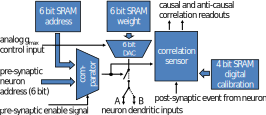
\includegraphics[width=\textwidth]{pictures/syncircuit.pdf}
    \caption{\label{fig:circuit} Block Diagram of the Synapse Circuit (modified from~\citeauthor{PPU}).}
\end{figure}
	\vspace*{-1em}
\begin{figure}
    \centering
    \begin{bytefield}[endianness=big, bitwidth=0.027777\linewidth, bitheight=2em]{32}
        \bitheader{0,7,15,23,31}\\
        \bitboxes{8}{{mnemonic}{operand}{operand}{operand}}\\
        \bitboxes{8}{{\tt{addi}}{{\tt r1} \\ \tiny register address}{{\tt r2} \\ \tiny register address}{{\tt 5} \\ \tiny immediate operand}}
    \end{bytefield}
    \caption{\label{fig:mnemonic} Representation of Assembly Instruction {\tt addi} as a Machine Instruction in Memory. The immediate value {\tt 5} is added to register {\tt r2} and the result written in {\tt r1}.}
\end{figure}

		\end{column}
		\begin{column}{.5\textwidth}

\begin{figure}
    \centering
    \includegraphics[width=\textwidth]{pictures/s2pp.pdf}
    \caption{\label{fig:s2pp} Detailed Structure of the s2pp Vector Extension (taken from~\citeauthor{PPU})}
\end{figure}
		\end{column}
	\end{columns}

\end{frame}
\begin{frame}[fragile]{Additional Figures}

\begin{figure}
	\vspace*{3em}
    \centering
	\begin{bytefield}[endianness=little, bitwidth=\widthof{\tiny bit}/2, bitheight=2em]{128}
        \bitheader{0,7,15,31,63,127}\\
    \bitboxes{8}{{QI}{\tiny Quarter \\ Integer}{}{}{}{}{}{}{}{}{}{}{}{}{}{}}\\
    \bitboxes{16}{{HI}{\tiny Half \\ Integer}{}{}{}{}{}{}}\\
	\bitboxes{32}{{SI}{\tiny Single \\ Integer}{}{}}\\
    \bitboxes{32}{{SF}{\tiny Single \\ Float}{}{}}\\
    \end{bytefield}
	\vspace*{-1.5em}
    \caption{\label{fig:vectorlength} Vector structures are 128 bits wide and split into common word sizes.}
\end{figure}

\begin{figure}
	\begin{bytefield}[endianness=little, bitheight=2em, bitwidth=\widthof{\tiny bit}]{32}
        \bitheader{0,1,7,15,31}\\
        \colorbitbox{lightgray}{1}{\tiny bit} && \bitbox{31}{}\\
        \colorbitbox{lightgray}{8}{byte} && \bitbox{24}{}\\
        \colorbitbox{lightgray}{16}{halfword} && \bitbox{16}{}\\
        \colorbitbox{lightgray}{32}{word}\\
    \end{bytefield}
	\vspace*{-1.5em}
    \caption{\label{fig:bitlength} Illustration of Word Sizes for 32-bit Words}
\end{figure}

\end{frame}

\end{document}
